\section{Expérimentation}

\subsection{Analyseur statique}

\begin{frame}{L'analyseur \texttt{ptrtype}}

    % TODO remplacer ça par le schéma penjili
    % TODO mentionner les annotations

\end{frame}

\begin{frame}{Traduction}
\begin{block}{Code C}
\insertcode{tc-c.c}
\end{block}

\only<1>{
\begin{block}{\langname}
\insertcode{tc-ml.c}
\end{block}
}

\only<2>{
\begin{block}{\langname + types inférés}
\insertcode{tc-ty.c}
\end{block}
}

\end{frame}

\subsection{Utilisation sur le noyau Linux}

\begin{frame}[fragile]{Code avec bug}
    % left bottom right top
    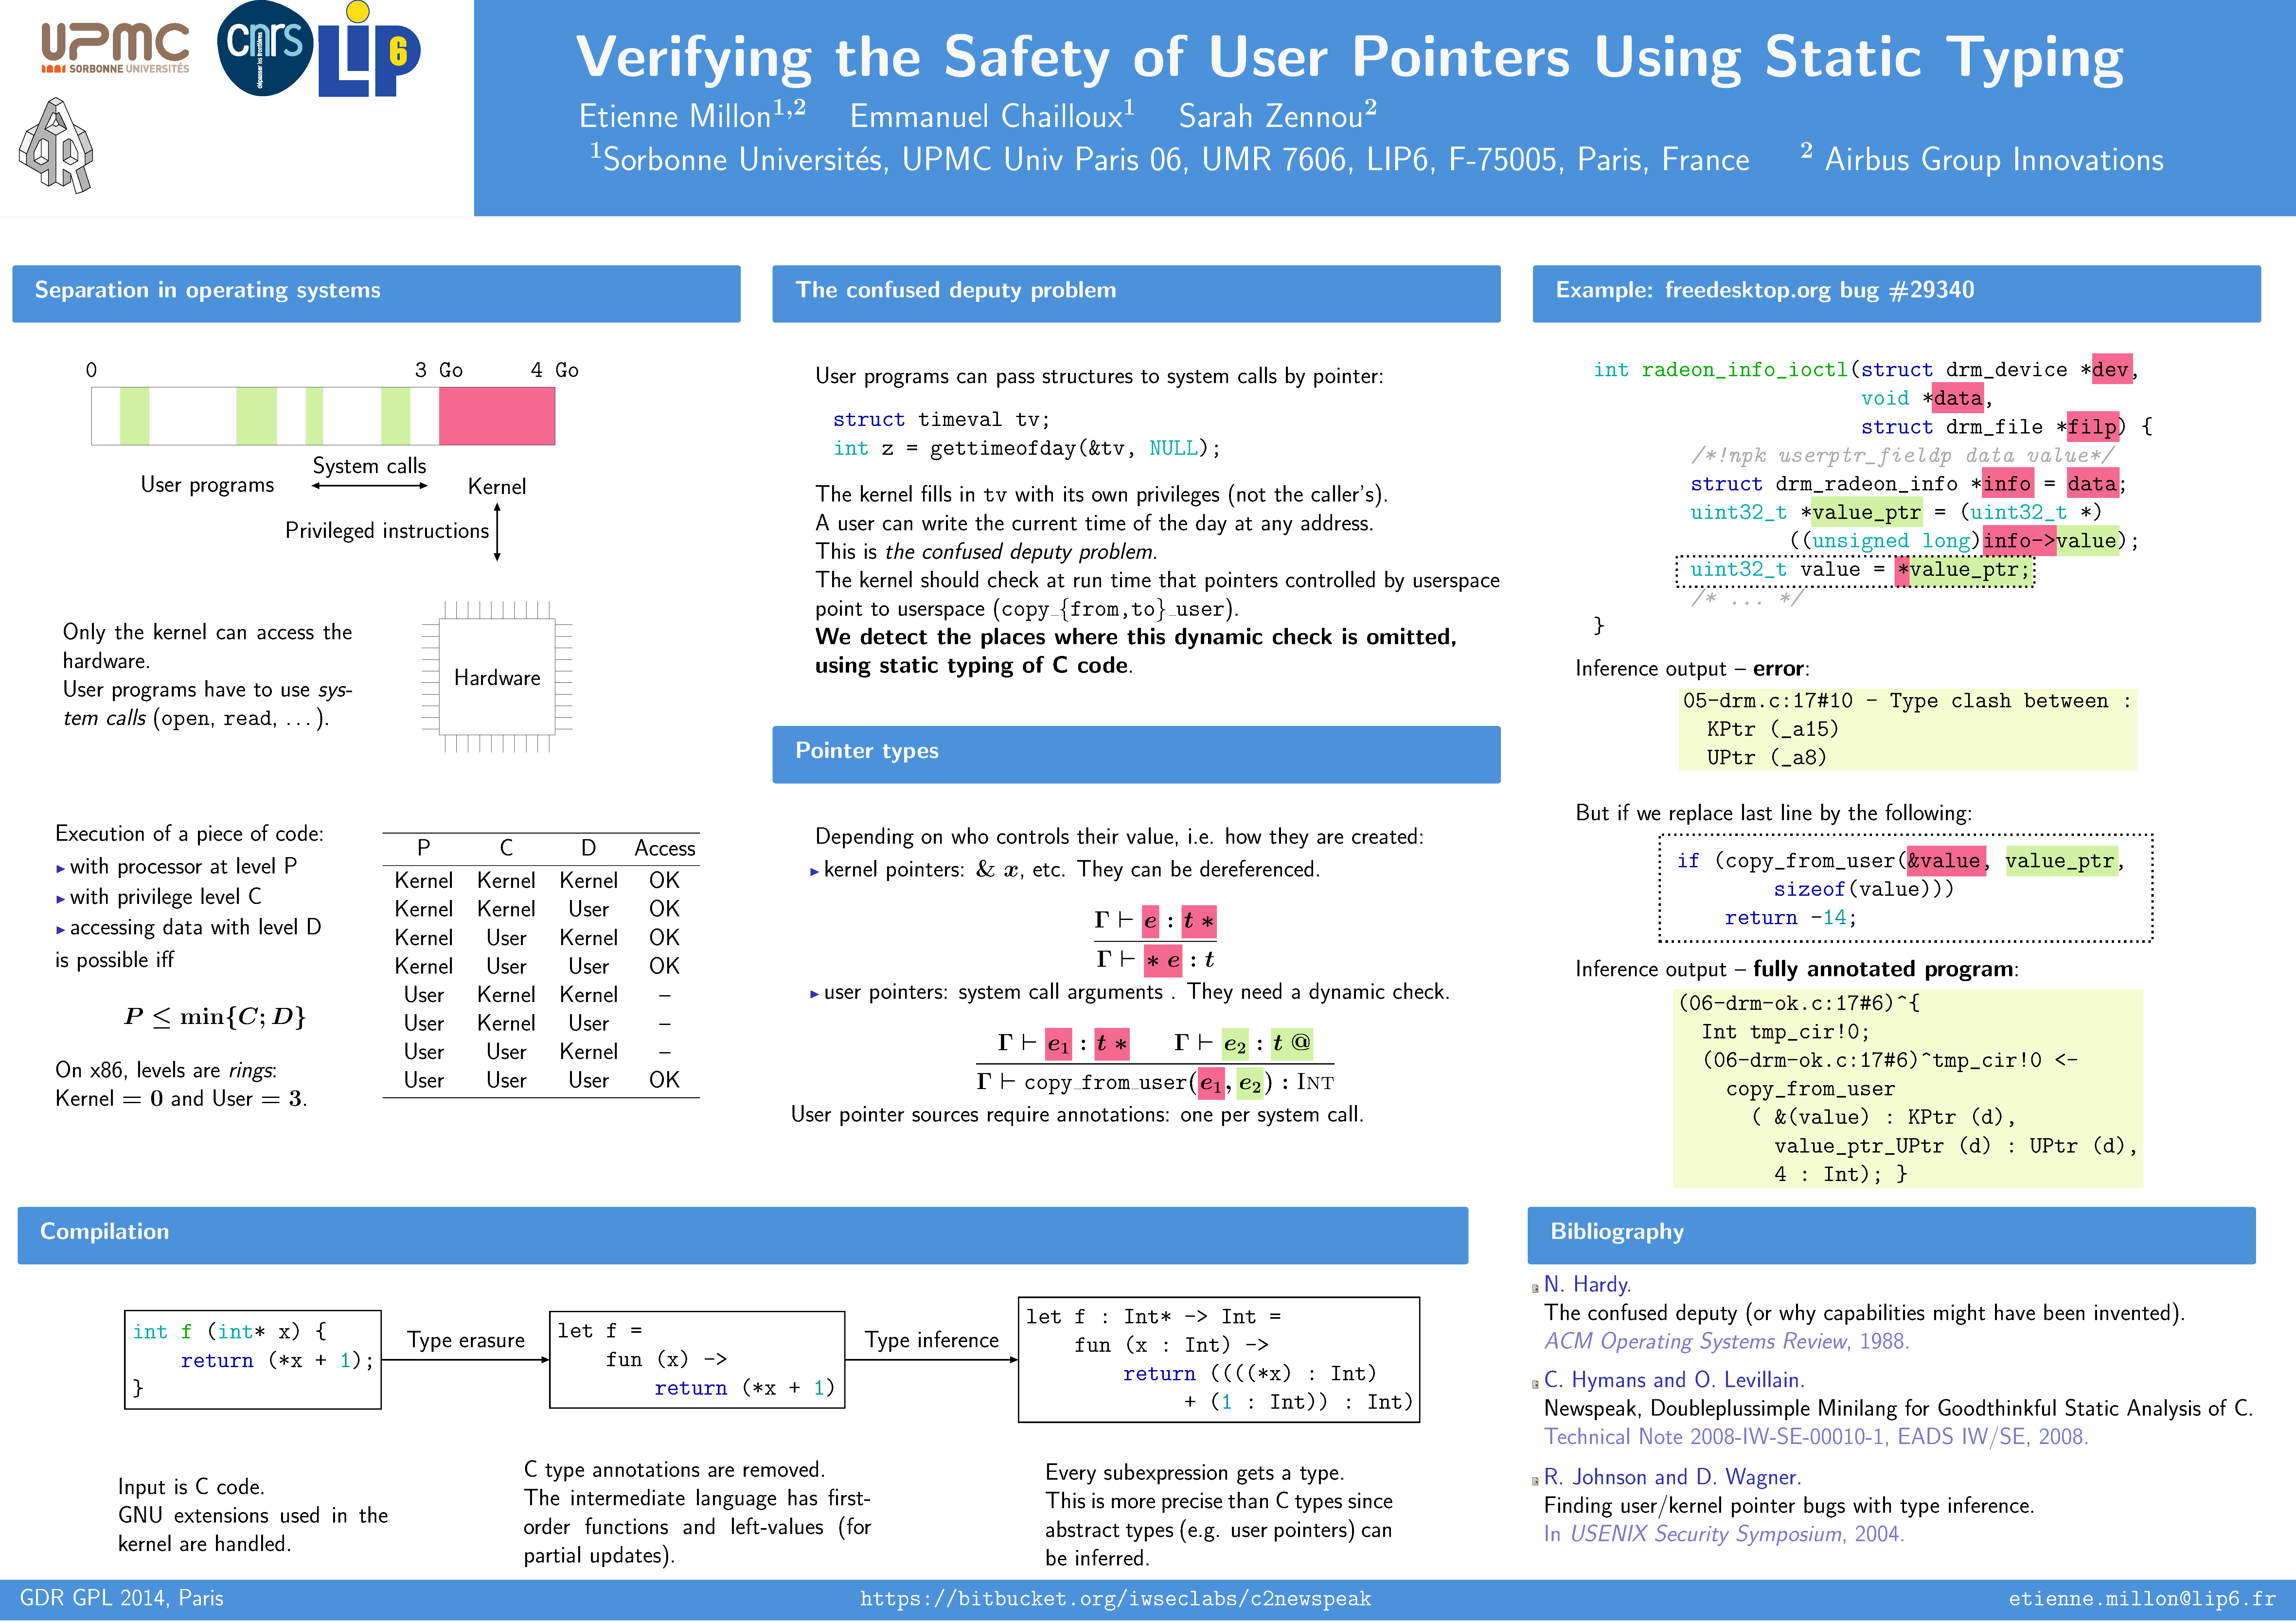
\includegraphics[trim=2300 1430 100 500,clip,width=\textwidth]{poster.pdf}

\begin{SaveVerbatim}{drmko}
05-drm.c:17#10 - Type clash between :
  KPtr (_a15)
  UPtr (_a8)
\end{SaveVerbatim}

% TODO impact de ce bug?

\codeout{drmko}
% ne pas parler des inconnues
\end{frame}

\begin{frame}{Code corrigé}
    % left bottom right top
    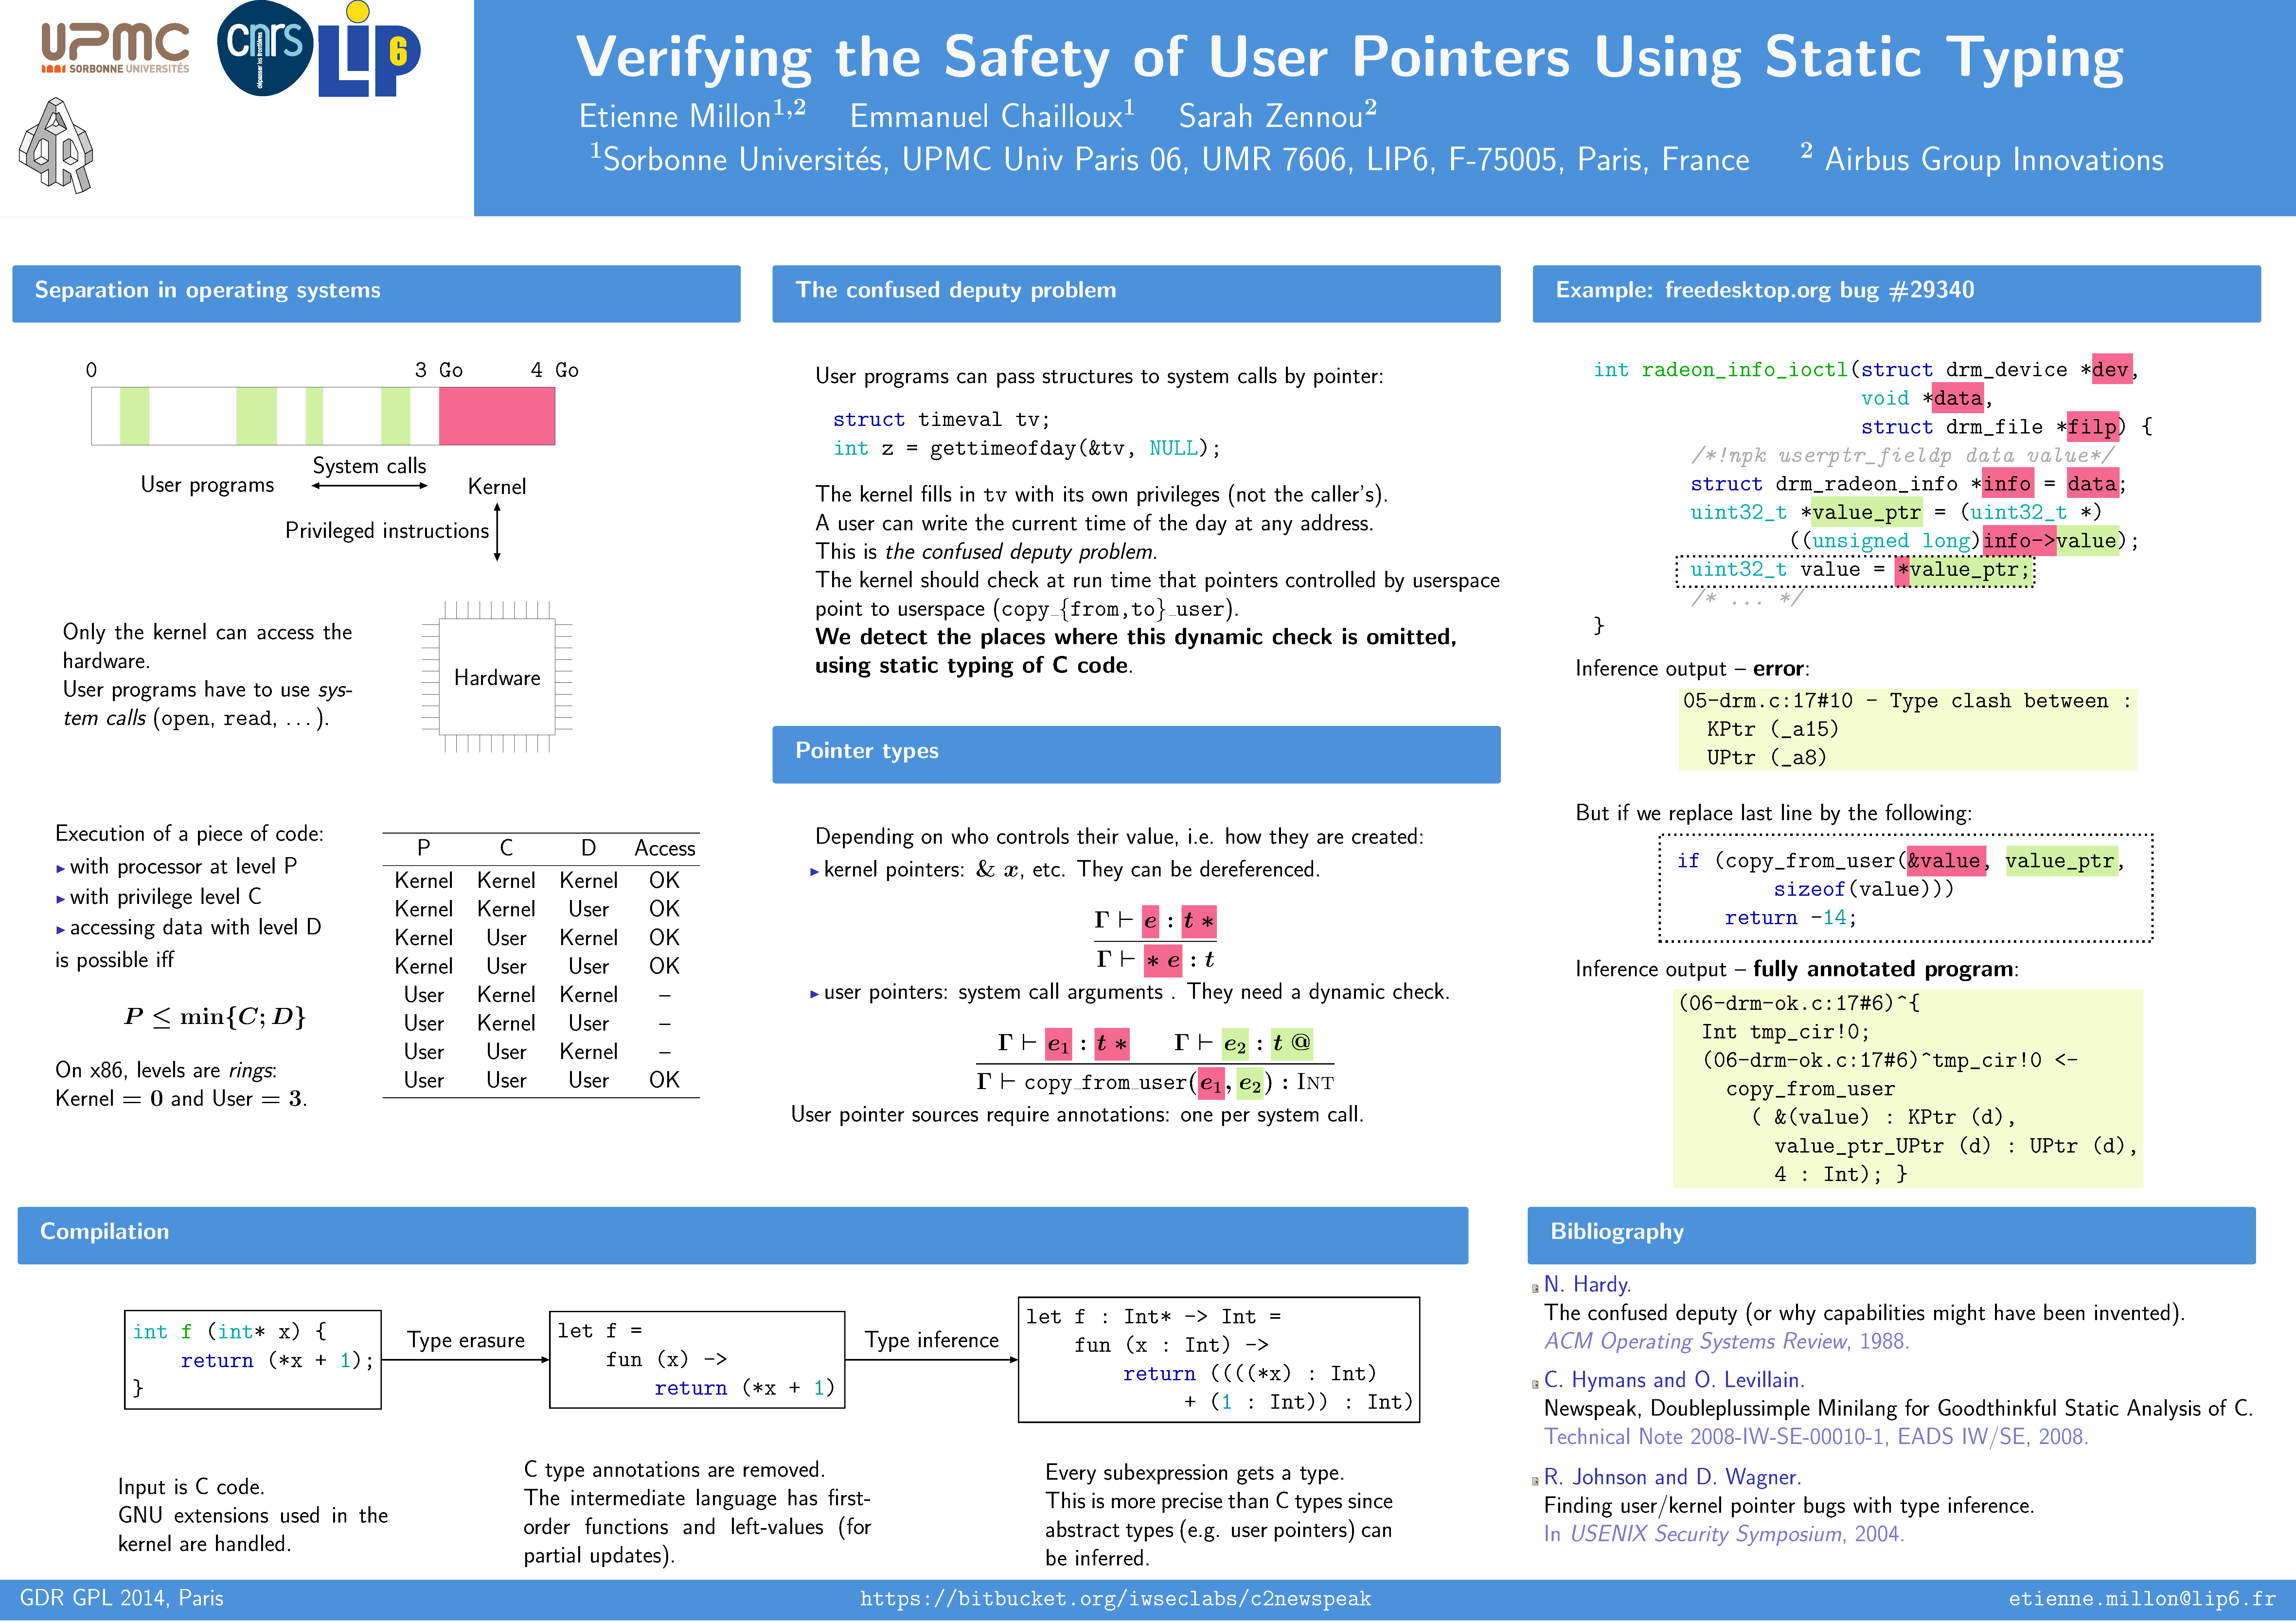
\includegraphics[trim=2300 990 100 1220,clip,width=\textwidth]{poster.pdf}
\end{frame}

\begin{frame}[fragile]{Résultat de l'algorithme d'inférence}

\textbf{Programme complètement étiqueté}:

\begin{SaveVerbatim}{drmok}
(06-drm-ok.c:17#6)^{
  Int tmp_cir!0;
  (06-drm-ok.c:17#6)^tmp_cir!0 <-
    copy_from_user
      ( &(value) : KPtr (d),
        value_ptr_UPtr (d) : UPtr (d),
        4 : Int); }
\end{SaveVerbatim}

\codeout{drmok}
\end{frame}
